\documentclass[../main.tex]{subfiles}
\begin{document}
Le espressioni regolari permetto di cercare delle sequenze di caratteri all'interno di stringhe di testo. Fino ad ora abbiamo visto ad
esempio il comando \code{grep}, tuttavia è piuttosto limitato. Per testare utilizzare il sito \code{regex101}.

\subsection{Pattern semplici}
\begin{itemize}
    \item \textbf{Singoli caratteri: } \code{b}, cerca il carattere b all'interno del testo
    \item \textbf{Sequenze di più caratteri: }, \code{mani} cerca la sequenza mani all'interno del testo (mani, romani, umani, ...)
\end{itemize}

\subsection{Caratteri speciali}
Alcuni caratteri assumono un significato speciale se sono preceduti da \code{\textbackslash}:
\begin{figure}[h]
    \centering
    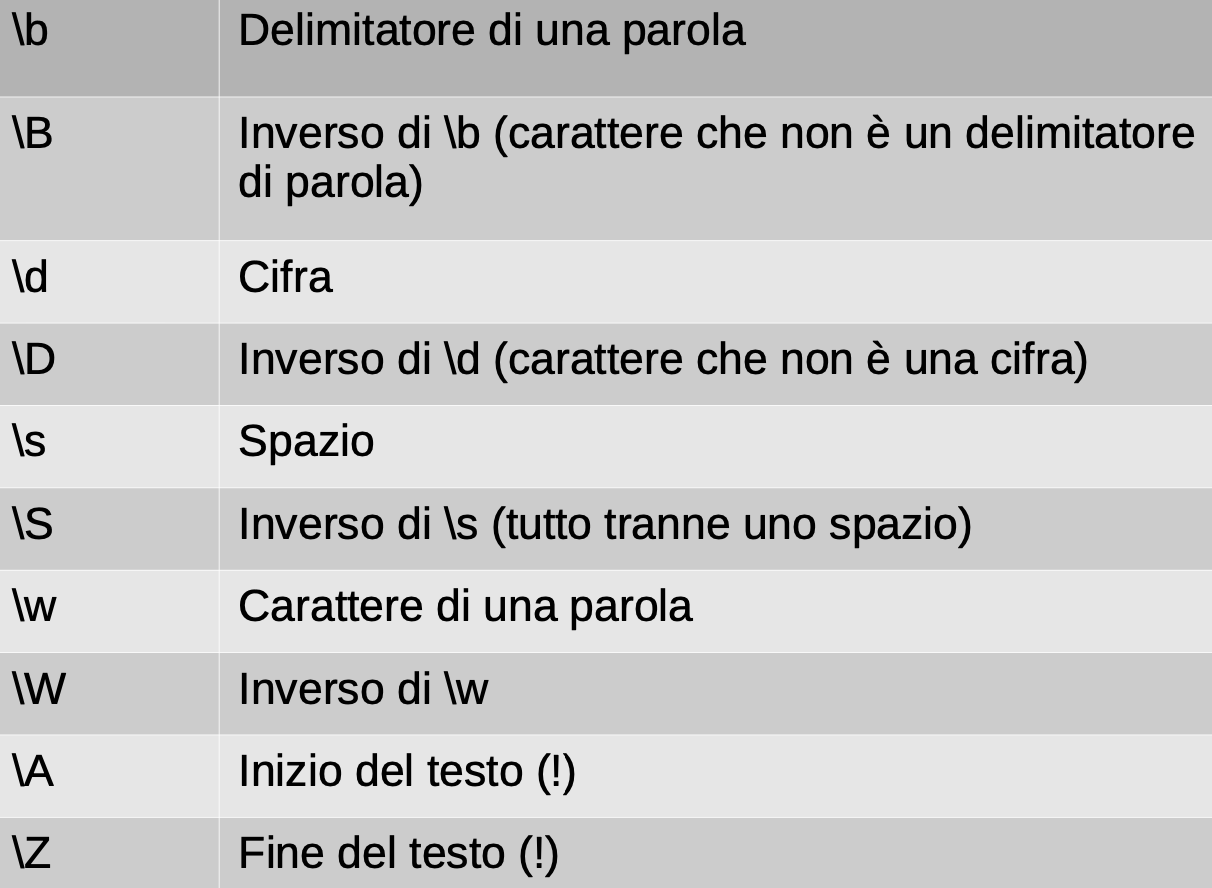
\includegraphics[width=0.5\textwidth]{../images/caratteriRegExp.png}
\end{figure}

\vspace{0.25cm}
Altri sono speciali senza l'utilizzo del \code{\textbackslash}:
\begin{figure}[h]
    \centering
    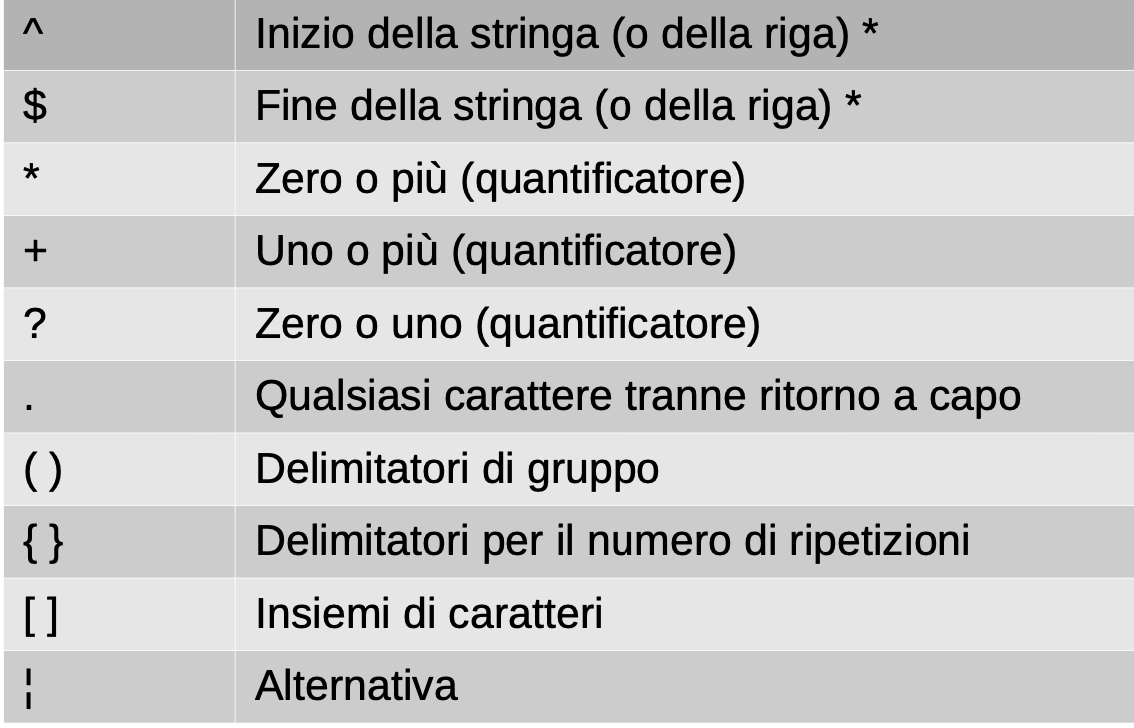
\includegraphics[width=0.5\textwidth]{../images/caratteriSpeciali.png}
\end{figure}

\textbf{Nota:} per trovare il carattere effettivo bisogna mettere prima \code{\textbackslash}, ad esempio \code{\textbackslash*}.

\vspace{0.5cm}
\subsubsection{Alternative}
Trova \code{ciao} oppure \code{cibo}, inoltre crea dei sottomatch per \code{ia} e \code{ib}.
\begin{lstlisting}[style=bash]
    c(ia | ib)o
\end{lstlisting}

\pagebreak
\subsection{Esempi}
Di base per cercare con le \code{regexp} usiamo \code{grep -E "regexp" a.txt}.

\begin{itemize}
    \item Trovare tutte le parole di un testo potremmo usare
    \begin{lstlisting}[style=bash]
        \b[A-Za-z]+\b
    
        #oppure
    
        \b[[:alpha:]]+\b
    \end{lstlisting}
    \item Trovare tutte le parole palindrome di quattro lettere
    \begin{lstlisting}[style=bash]
        \b(\w)(\w)\2\1\b
    \end{lstlisting}
\end{itemize}



\end{document}